\documentclass{standalone}
\usepackage{tikz}
\usepackage{ctex,siunitx}
\setCJKmainfont{Noto Serif CJK SC}
\usepackage{tkz-euclide}
\usepackage{amsmath}
\usetikzlibrary{patterns, calc,3d}
\usetikzlibrary {decorations.pathmorphing,decorations.pathreplacing,decorations.shapes}
\begin{document}
\small
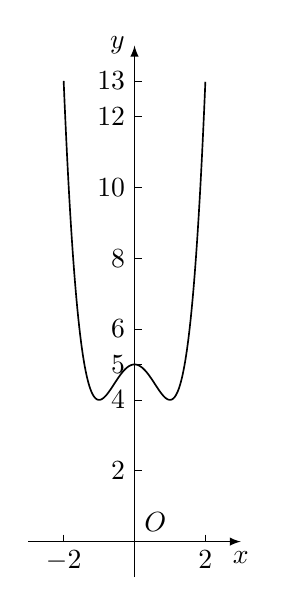
\begin{tikzpicture}[>=latex,scale=0.45]
  \draw[->](-3,0)--(3,0)node[below]{$x$};
  \draw[->](0,-1)--(0,14)node[left]{$y$};
  \node at (0,0)[above right]{$O$};
  \draw[samples=200,domain=-2:2,semithick]plot(\x,{\x*\x*\x*\x-2*\x*\x+5});
  \foreach \x in{-2,2}
  {
    \draw[very thin](\x,0.2)--(\x,0)node[below]{$\x$};
  }
  \foreach \y in {2,4,5,6,8,10,12,13}
  {
    \draw[very thin](0.2,\y)--(0,\y)node[left]{$\y$};
  }
\end{tikzpicture}
\end{document}